% Generated by extension/cross_study/make_assets.py. Do not edit.
\definecolor{donorcol}{HTML}{5D6670}
\definecolor{haocol}{HTML}{217D91}
\definecolor{coloncol}{HTML}{A64442}
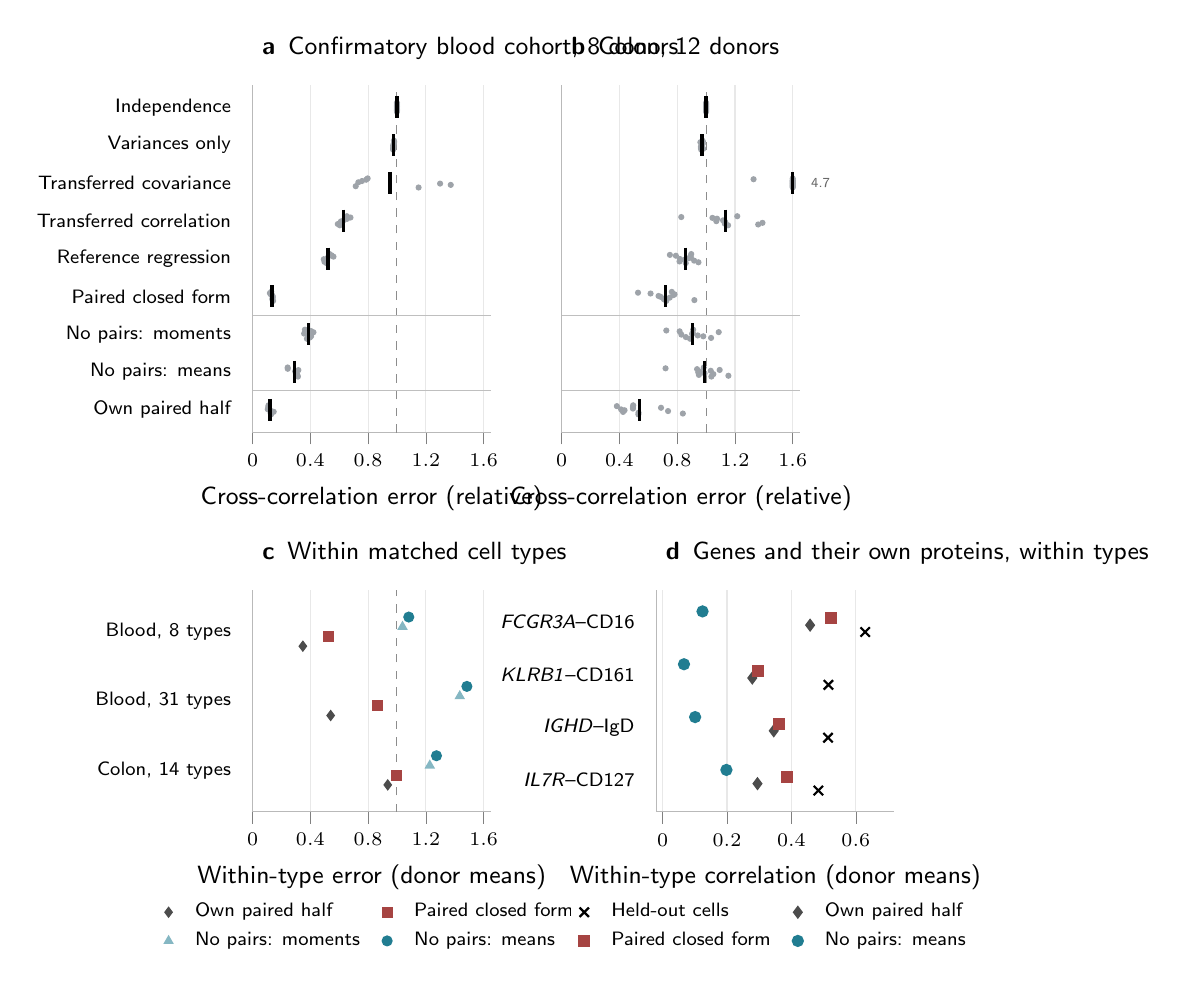
\begin{tikzpicture}[font=\sffamily]
\begin{axis}[name=a,width=.38\textwidth,height=6.0cm,xmin=0,xmax=1.6500000000000001,ymin=.4,ymax=9.6,
 xtick={0,.4,.8,1.2,1.6},ytick={1,2,3,4,5,6,7,8,9},yticklabels={{Own paired half},{No pairs: means},{No pairs: moments},{Paired closed form},{Reference regression},{Transferred correlation},{Transferred covariance},{Variances only},{Independence}},
 xlabel={Cross-correlation error (relative)},title={\textbf{a}\enspace Confirmatory blood cohort, 8 donors},
 axis x line*=bottom,axis y line*=left,tick align=outside,y tick style={draw=none},xmajorgrids=true,grid style={gray!18},axis line style={gray!55},tick label style={font=\sffamily\scriptsize},label style={font=\sffamily\small},clip=false,title style={font=\sffamily\small,at={(0,1)},anchor=base west,yshift=5pt}]
\draw[dashed,black!45] (axis cs:1,.4) -- (axis cs:1,9.6);
\draw[black!25] (axis cs:0,1.5) -- (axis cs:1.6500000000000001,1.5);
\draw[black!25] (axis cs:0,3.5) -- (axis cs:1.6500000000000001,3.5);
\addplot[only marks,mark=*,mark size=.9pt,color=donorcol!60] coordinates {
 (0.1282,0.880) (0.1256,0.914) (0.1467,0.949) (0.1235,0.983) (0.1057,1.017) (0.1105,1.051) (0.1095,1.086) (0.1112,1.120)
 (0.3142,1.880) (0.3108,1.914) (0.3052,1.949) (0.3030,1.983) (0.2952,2.017) (0.3175,2.051) (0.2438,2.086) (0.2433,2.120)
 (0.3767,2.880) (0.3977,2.914) (0.4060,2.949) (0.3868,2.983) (0.3572,3.017) (0.4217,3.051) (0.4035,3.086) (0.3627,3.120)
 (0.1424,3.880) (0.1377,3.914) (0.1383,3.949) (0.1401,3.983) (0.1385,4.017) (0.1271,4.051) (0.1203,4.086) (0.1295,4.120)
 (0.5121,4.880) (0.4982,4.914) (0.5156,4.949) (0.4934,4.983) (0.5196,5.017) (0.5605,5.051) (0.5470,5.086) (0.5334,5.120)
 (0.6046,5.880) (0.5906,5.914) (0.6106,5.949) (0.6123,5.983) (0.6325,6.017) (0.6550,6.051) (0.6782,6.086) (0.6533,6.120)
 (1.1499,6.880) (0.7146,6.914) (1.3725,6.949) (1.2988,6.983) (0.7328,7.017) (0.7581,7.051) (0.7870,7.086) (0.7972,7.120)
 (0.9736,7.880) (0.9734,7.914) (0.9753,7.949) (0.9742,7.983) (0.9765,8.017) (0.9785,8.051) (0.9808,8.086) (0.9792,8.120)
 (1.0000,8.880) (1.0000,8.914) (1.0000,8.949) (1.0000,8.983) (1.0000,9.017) (1.0000,9.051) (1.0000,9.086) (1.0000,9.120)};
\addplot[only marks,mark=|,mark size=4pt,line width=1.2pt,color=black] coordinates { (0.1201,1) (0.2916,2) (0.3890,3) (0.1342,4) (0.5225,5) (0.6297,6) (0.9514,7) (0.9764,8) (1.0000,9) };
\end{axis}
\begin{axis}[at={(a.east)},anchor=west,xshift=0.9cm,name=b,width=.38\textwidth,height=6.0cm,xmin=0,xmax=1.6500000000000001,ymin=.4,ymax=9.6,
 xtick={0,.4,.8,1.2,1.6},ytick={1,2,3,4,5,6,7,8,9},yticklabels={},
 xlabel={Cross-correlation error (relative)},title={\textbf{b}\enspace Colon, 12 donors},
 axis x line*=bottom,axis y line*=left,tick align=outside,y tick style={draw=none},xmajorgrids=true,grid style={gray!18},axis line style={gray!55},tick label style={font=\sffamily\scriptsize},label style={font=\sffamily\small},clip=false,title style={font=\sffamily\small,at={(0,1)},anchor=base west,yshift=5pt}]
\draw[dashed,black!45] (axis cs:1,.4) -- (axis cs:1,9.6);
\draw[black!25] (axis cs:0,1.5) -- (axis cs:1.6500000000000001,1.5);
\draw[black!25] (axis cs:0,3.5) -- (axis cs:1.6500000000000001,3.5);
\addplot[only marks,mark=*,mark size=.9pt,color=donorcol!60] coordinates {
 (0.5314,0.880) (0.8391,0.902) (0.5322,0.924) (0.4251,0.945) (0.7367,0.967) (0.4353,0.989) (0.4115,1.011) (0.4936,1.033) (0.6879,1.055) (0.4936,1.076) (0.3822,1.098) (0.4952,1.120)
 (1.0367,1.880) (1.1545,1.902) (0.9502,1.924) (1.0503,1.945) (0.9895,1.967) (0.9459,1.989) (0.9586,2.011) (1.0323,2.033) (1.0941,2.055) (0.9376,2.076) (0.7193,2.098) (0.9841,2.120)
 (0.8887,2.880) (1.0346,2.902) (0.8601,2.924) (0.9805,2.945) (0.9421,2.967) (0.8289,2.989) (0.9034,3.011) (0.9082,3.033) (1.0875,3.055) (0.8169,3.076) (0.7244,3.098) (0.9105,3.120)
 (0.7242,3.880) (0.9190,3.902) (0.7080,3.924) (0.7136,3.945) (0.7482,3.967) (0.6851,3.989) (0.6709,4.011) (0.7731,4.033) (0.7814,4.055) (0.6156,4.076) (0.5286,4.098) (0.7626,4.120)
 (0.8591,4.880) (0.9472,4.902) (0.8161,4.924) (0.9173,4.945) (0.8501,4.967) (0.8188,4.989) (0.8808,5.011) (0.8937,5.033) (0.8929,5.055) (0.7910,5.076) (0.7495,5.098) (0.8971,5.120)
 (1.1522,5.880) (1.3608,5.902) (1.1296,5.924) (1.3904,5.945) (1.1323,5.967) (1.0708,5.989) (1.1174,6.011) (1.0724,6.033) (1.0758,6.055) (1.0440,6.076) (0.8282,6.098) (1.2158,6.120)
 (1.6000,6.880) (1.6000,6.902) (1.6000,6.924) (1.6000,6.945) (1.6000,6.967) (1.6000,6.989) (1.6000,7.011) (1.6000,7.033) (1.6000,7.055) (1.6000,7.076) (1.3288,7.098) (1.6000,7.120)
 (0.9662,7.880) (0.9799,7.902) (0.9646,7.924) (0.9732,7.945) (0.9647,7.967) (0.9696,7.989) (0.9735,8.011) (0.9756,8.033) (0.9759,8.055) (0.9605,8.076) (0.9773,8.098) (0.9744,8.120)
 (1.0000,8.880) (1.0000,8.902) (1.0000,8.924) (1.0000,8.945) (1.0000,8.967) (1.0000,8.989) (1.0000,9.011) (1.0000,9.033) (1.0000,9.055) (1.0000,9.076) (1.0000,9.098) (1.0000,9.120)};
\addplot[only marks,mark=|,mark size=4pt,line width=1.2pt,color=black] coordinates { (0.5387,1) (0.9878,2) (0.9072,3) (0.7192,4) (0.8595,5) (1.1325,6) (1.6000,7) (0.9713,8) (1.0000,9) };
\node[font=\sffamily\tiny,anchor=west,black!60] at (axis cs:1.6600000000000001,7) {4.7};
\end{axis}
\begin{axis}[at={(a.south west)},anchor=north west,yshift=-2.0cm,name=c,
 width=.38\textwidth,height=4.4cm,xmin=0,xmax=1.6500000000000001,ymin=.4,ymax=3.6,
 xtick={0,.4,.8,1.2,1.6},ytick={1,2,3},yticklabels={{Colon, 14 types},{Blood, 31 types},{Blood, 8 types}},
 xlabel={Within-type error (donor means)},
 title={\textbf{c}\enspace Within matched cell types},
 axis x line*=bottom,axis y line*=left,tick align=outside,y tick style={draw=none},xmajorgrids=true,grid style={gray!18},axis line style={gray!55},tick label style={font=\sffamily\scriptsize},label style={font=\sffamily\small},clip=false,title style={font=\sffamily\small,at={(0,1)},anchor=base west,yshift=5pt},
 legend style={draw=none,font=\sffamily\scriptsize,at={(0.5,-0.36)},anchor=north,legend columns=2,cells={anchor=west},column sep=6pt}]
\draw[dashed,black!45] (axis cs:1,.4) -- (axis cs:1,3.6);
\addplot[only marks,mark=diamond*,mark size=1.8pt,color=black!70] coordinates { (0.9362,0.790) (0.5411,1.790) (0.3485,2.790) };
\addlegendentry{Own paired half}
\addplot[only marks,mark=square*,mark size=1.8pt,color=coloncol] coordinates { (0.9997,0.930) (0.8684,1.930) (0.5280,2.930) };
\addlegendentry{Paired closed form}
\addplot[only marks,mark=triangle*,mark size=1.8pt,color=haocol!55] coordinates { (1.2274,1.070) (1.4350,2.070) (1.0385,3.070) };
\addlegendentry{No pairs: moments}
\addplot[only marks,mark=*,mark size=1.8pt,color=haocol] coordinates { (1.2737,1.210) (1.4844,2.210) (1.0820,3.210) };
\addlegendentry{No pairs: means}
\end{axis}
\begin{axis}[at={(c.east)},anchor=west,xshift=2.1cm,name=d,
 width=.38\textwidth,height=4.4cm,xmin=-.02,xmax=.72,ymin=.4,ymax=4.6,
 xtick={0,.2,.4,.6},ytick={1,2,3,4},yticklabels={{\textit{IL7R}--CD127},{\textit{IGHD}--IgD},{\textit{KLRB1}--CD161},{\textit{FCGR3A}--CD16}},
 xlabel={Within-type correlation (donor means)},
 title={\textbf{d}\enspace Genes and their own proteins, within types},
 axis x line*=bottom,axis y line*=left,tick align=outside,y tick style={draw=none},xmajorgrids=true,grid style={gray!18},axis line style={gray!55},tick label style={font=\sffamily\scriptsize},label style={font=\sffamily\small},clip=false,title style={font=\sffamily\small,at={(0,1)},anchor=base west,yshift=5pt},
 legend style={draw=none,font=\sffamily\scriptsize,at={(0.5,-0.36)},anchor=north,legend columns=2,cells={anchor=west},column sep=6pt}]
\addplot[only marks,mark=x,mark size=2.4pt,color=black,line width=.8pt] coordinates { (0.4838,0.805) (0.5137,1.805) (0.5150,2.805) (0.6291,3.805) };
\addlegendentry{Held-out cells}
\addplot[only marks,mark=diamond*,mark size=1.8pt,color=black!70,line width=.8pt] coordinates { (0.2947,0.935) (0.3452,1.935) (0.2785,2.935) (0.4581,3.935) };
\addlegendentry{Own paired half}
\addplot[only marks,mark=square*,mark size=1.8pt,color=coloncol,line width=.8pt] coordinates { (0.3869,1.065) (0.3607,2.065) (0.2963,3.065) (0.5230,4.065) };
\addlegendentry{Paired closed form}
\addplot[only marks,mark=*,mark size=1.8pt,color=haocol,line width=.8pt] coordinates { (0.1982,1.195) (0.1010,2.195) (0.0664,3.195) (0.1240,4.195) };
\addlegendentry{No pairs: means}
\end{axis}
\end{tikzpicture}
